% !TEX program = lualatex
\documentclass[8pt,twocolumn]{article}

% Essential packages
\usepackage{mdframed}
\usepackage{xcolor}

% Define a nice framed box for the abstract
\definecolor{lightgray}{gray}{0.95}
\newenvironment{abstractbox}{%
  \begin{mdframed}[backgroundcolor=lightgray,
                   linewidth=0.5pt,
                   linecolor=black,
                   topline=true,
                   bottomline=true,
                   leftline=true,
                   rightline=true,
                   innerleftmargin=10pt,
                   innerrightmargin=10pt,
                   innertopmargin=10pt,
                   innerbottommargin=10pt]
}{%
  \end{mdframed}
}

% Essential packages
\usepackage{fontspec}        % Font selection for LuaLaTeX
\usepackage{amsmath,amssymb} % Math symbols and environments
\usepackage{graphicx}        % For including images
\usepackage{booktabs}        % For professional tables
\usepackage{hyperref}        % For hyperlinks
\usepackage{geometry}        % For page layout
\usepackage{algorithm}       % For algorithms
\usepackage{algpseudocode} % For algorithm pseudocode

% BIBLIOGRAPHY SETTINGS
\usepackage[numbers]{natbib}    
\bibliographystyle{IEEEtran}

% Page layout
\geometry{
  paper=a4paper,
  top=0.5cm,
  bottom=1.0cm,
  left=0.5cm,
  right=0.5cm,
}

\usepackage{fancyhdr}
\pagestyle{fancy}
\fancyhf{} % Clear all header and footer fields
\fancyfoot[C]{\thepage} % Page number at center of footer
\renewcommand{\headrulewidth}{0pt} % Remove header rule
\setlength{\footskip}{15pt} % Increase this value to move page number up

% Remove large paragraph indents
\setlength{\parindent}{0pt}   % Remove paragraph indentation completely
\setlength{\parskip}{0.1cm}   % Add some vertical space between paragraphs

\setmainfont{TeX Gyre Termes}[
  Ligatures=TeX,
  Numbers=OldStyle
]

% Section styling
\usepackage{titlesec}

% Format section headings
\titleformat{\section}
  {\normalfont\large\bfseries}  % format
  {\thesection}                 % label
  {1em}                         % sep
  {\MakeUppercase}              % before-code
  []                            % after-code

% Adjust spacing around sections
\titlespacing*{\section}
  {0pt}                         % left
  {1.5ex plus .5ex minus .2ex}  % before
  {1ex plus .2ex} 


% Font settings - using TeX Gyre Termes (Times-like font) for maximum compatibility
\usepackage{fontspec}
\setmainfont{TeX Gyre Termes}[
  Ligatures=TeX,
  Numbers=OldStyle
]

% Hyperref settings
\hypersetup{
  colorlinks=true,
  linkcolor=black,
  citecolor=black,
  urlcolor=black,
}

% Title information
\title{\textbf{Non-Linear Regression: comparison between P-Splines and SVM Regression Using Sine-Exponential Simulated Data}}
\author{First Author and Second Author\\
}
\date{}

\begin{document}

\maketitle

\begin{abstractbox}
\noindent\textbf{Abstract} \\
DO NOT FORGET TO INCLUDE SECTION HERE!!!

\vspace{0.5em}
\noindent\textbf{KEY WORDS:} \ non-linear regression; GAM; univariate analysis; P-Splines; SVM Regression; simulation study
\end{abstractbox}


% 1. INTRODUCTION
\section{INTRODUCTION}

There has been a significant development in non-linear regression techniques due to the advent of modern high-speed computing.
This new family of techniques, often originating from machine learning and computer science environments directly compete with
more traditional statistics techniques whose theory predates the contemporary machine learning algorithm.

This simulation study aims to compare two such techniques: Splines which have origins in 20th century, and the Support Vector Machines that became
a technique-of-choice in the early 21st century before neural networks became more viable option in recent years.

\subsection{Splines}

Splines were first proposed in 1946 by Schoenberg who provided mathematical theory
for piecewise polynomial functions that are connected via knots \cite{schoenberg1946}. This was later improved by
the introduction of smoothing splines in 1967 by Reinsch for balancing smoothness with data fitting \cite{reinchs1967}.

However, the previous approaches relied on subjective parameter selection. The
key development came with the introduction of generalised cross-validation in 1978 \cite{crwah1978}.
Smoothing spline theory as well as cubic splines were then formalused by Wahba in 1990 \cite{wahba1990}.

At the same time, there was a development in an alternative approach using basis splines (B-splines)
that, due to them using local rather than global support, are computationally more efficient \cite{deboor1978}.
However, B-splines require manual knot placement and selection which makes their
use more subjective and prone to errors in practice.

The key development that brought splines to prominance was Eilers and Marx's introduction
of penalised B-splines (P-splines) in 1996 \cite{eilmarx1996}. The technique combines computational
efficiency of B-splines with the adaptive smoothing penalty techniques. Due to its use of large
number of equally-spced knots. The penalty is then applied between adjacing B-spline coefficients.
This approach balances smoothness and fit through a single tuning parameter and avoids a subjective choice
of knot locations. However, the number of appropriate knots still remains subjective with larger number
of knots may still lead to overfitting, albeit much less pronounced compared to B-splines.

The contemporary developments include the introduction of both frequentist \cite{krivo2008} and
Bayesian \cite{woods2017} uncertainty quantification which allowed for scientific applcation of splines. There has also been
significant development in other fields, such as multivariate extensions and functional data analysis \cite{woods2017}

The univariate P-spline model uses the following two equations:

\begin{equation}
    f(x) = \sum_{j=1}^{n} \beta_j B_j(x)
\end{equation}

where $B_j(x)$ are B-spline basis functions; $\beta_j$ are coefficients;
and $n$ is the number of basis functions.

The above is subject to the following minimisation contraint for coefficient estimation:
\begin{equation}
    \sum_{i=1}^{m} (y_i - f(x_i))^2 + \lambda \sum_{j=d+1}^{n} (\Delta^d \beta_j)^2
\end{equation}

where the first term measures fit to the data; the second term is a penalty on differences between adjacent coefficients;
$\lambda$ is the smoothing parameter; and $\Delta^d$ represents the $d$ order difference operator.


\subsection{Support Vector Reggresion}
Vapnik \cite{vapnik1995nature} proposed the Support Vector Regression (SVR) framework
by extending Support Vector Machine (SVM) to regression models. SVR constructs a
regression function based on a subset of the data, known as support vectors. In its original form, Vapnik introduced the following representation:

\begin{equation}
F_2(x, \mathbf{w}) = \sum_{i=1}^{N} (\alpha_i^* - \alpha_i) (v_i^\top x + 1)^p + b
\end{equation}

Here, $\alpha_i$, $\alpha_i^*$ are Lagrange multipliers obtained from the dual optimization
problem, $v_i$ represents the data samples, $p$ is the degree of the polynomial kernel, and the term $(v_i^\top x + 1)^p$ corresponds to the kernel
function. This formula use a specific polinomial kernel.

The SVR model can be more generalized replacing the polynomial kernel with any positive-definite
kernel function $K(x_i, x)$, leading to the more flexible representation:

\begin{equation}
f(x) = \sum_{i=1}^{N} (\alpha_i^* - \alpha_i) K(x_i, x) + b
\end{equation}

This form allows SVR to capture complex, non-linear relationships in data.
Commonly used kernels include the radial basis function, linear and sigmoid kernels,
making SVR a powerful and adaptable tool for regression tasks involving non-linear data structures.

\subsubsection{Loss Function and Hyperparameters}
The loss function utilized in this model is the $\varepsilon$-insensitive loss function, first
introduced by Vapnik \cite{vapnik1995nature}. This loss function defines a tube of tolerance around the regression function,
within which errors are not penalized. The idea is to focus on fitting the data while ignoring small deviations that
are likely due to noise (just like the svm do to separed classes). The loss function $L_\varepsilon$ is defined as:

\begin{equation}
L_\varepsilon(y, f(x)) = 
\begin{cases}
0, & \text{if } |y - f(x)| \leq \varepsilon \\
|y - f(x)| - \varepsilon, & \text{otherwise}
\end{cases}
\end{equation}

Only data points that lie outside the $\varepsilon$-tube contribute to
the cost function, making the solution sparse in terms of support vectors \cite{smola1998tutorial}.

The Hyperparameters that are involve in this model are three and they are use to control
the flexibility and generalization of the model:

\begin{itemize}
    \item \textbf{Regularization parameter $C$}: This controls the bias-variance trade-off of the model. A high $C$ encourages the model to minimize errors at the risk of overfitting, while a small $C$ yields a smoother function that may tolerate larger errors.
    \item \textbf{Epsilon $\varepsilon$}: Determines the width of the tube around the regression function where no penalty is applied. Larger values of $\varepsilon$ simplify the model by ignoring small deviations, while smaller values increase sensitivity to minor variations.
    \item \textbf{Kernel function $K(x_i, x_j)$}: Enables SVR to perform non-linear regression by implicitly mapping the input data into a higher-dimensional feature space. Common kernel choices include:
    \begin{itemize}
        \item \textit{Linear}: $K(x_i, x_j) = x_i^\top x_j$
        \item \textit{Polynomial}: $K(x_i, x_j) = (\gamma x_i^\top x_j + r)^d$
        \item \textit{Radial Basis Function (RBF)}: $K(x_i, x_j) = \exp(-\gamma \|x_i - x_j\|^2)$
        \item \textit{Sigmoid}: $K(x_i, x_j) = \tanh(\gamma x_i^\top x_j + r)$
    \end{itemize}
\end{itemize}

As noted by Hastie \emph{et al.} \cite{hastie2009elements}, the choice and tuning of these hyperparameters are crucial for model performance and are selected through cross-validation techniques.


\section{Simulation Study}

This section discusses the specific apporach that was taken for the simulation
study, decisions taken regarding each implementation, and presentation of final
comparison results:

\subsection{Methodology}

\subsubsection{Data Simulation}

To evaluate the performance, sine-exponential function was used to simulate data.
This nonlinear function combines periodic oscillations with exponential growth, creating a
challenging test case for nonparametric regression techniques.

The underlying deterministic function is defined as:

$$f(x) = \sin(x) \cdot e^{\alpha x}$$

where $\alpha = 0.2$ represents the exponential growth rate parameter.
The complete data generating process is formalised as:

$$y_i = \sin(x_i) \cdot e^{0.2x_i} + \varepsilon_i, \quad i = 1,\ldots,n$$

with the following specifications:$x_i \sim \mathcal{U}(0, 6\pi)$ (\emph{random sampling specification};
$\varepsilon_i \sim \mathcal{N}(0, \sigma^2)$, where $\sigma = 10$ represents the standard deviation of Gaussian noise; and
$n = 1000$ represents the total number of observations.

\subsubsection{P-Spline Implementation}

P-spline model was implemented using \textbf{mgcv} package that is from Wood \cite{mgcv} and is still activelly developed.
The package includes automatic GCV which was used for smoothing parameter tuning.
According to Woods \cite{woods2017} second-order difference penalty is best choice for fitting
a data with oscillating pattern and therefore was used in our model specification.

However, the choice of number of knots is still subjective and relative to data. Based on
graphical analysis, the appropriate number of knots was determined to be 40. Despite the overlapping with
its double, 40 was chosen due to its reduced complexity. However, the effective degrees of freedom (EDF) is 16.159 meaning the number of knots was effectively reduced to prevent overfitting which suggest the penalisation function works as intended.

\begin{figure}[htbp]
    \centering
    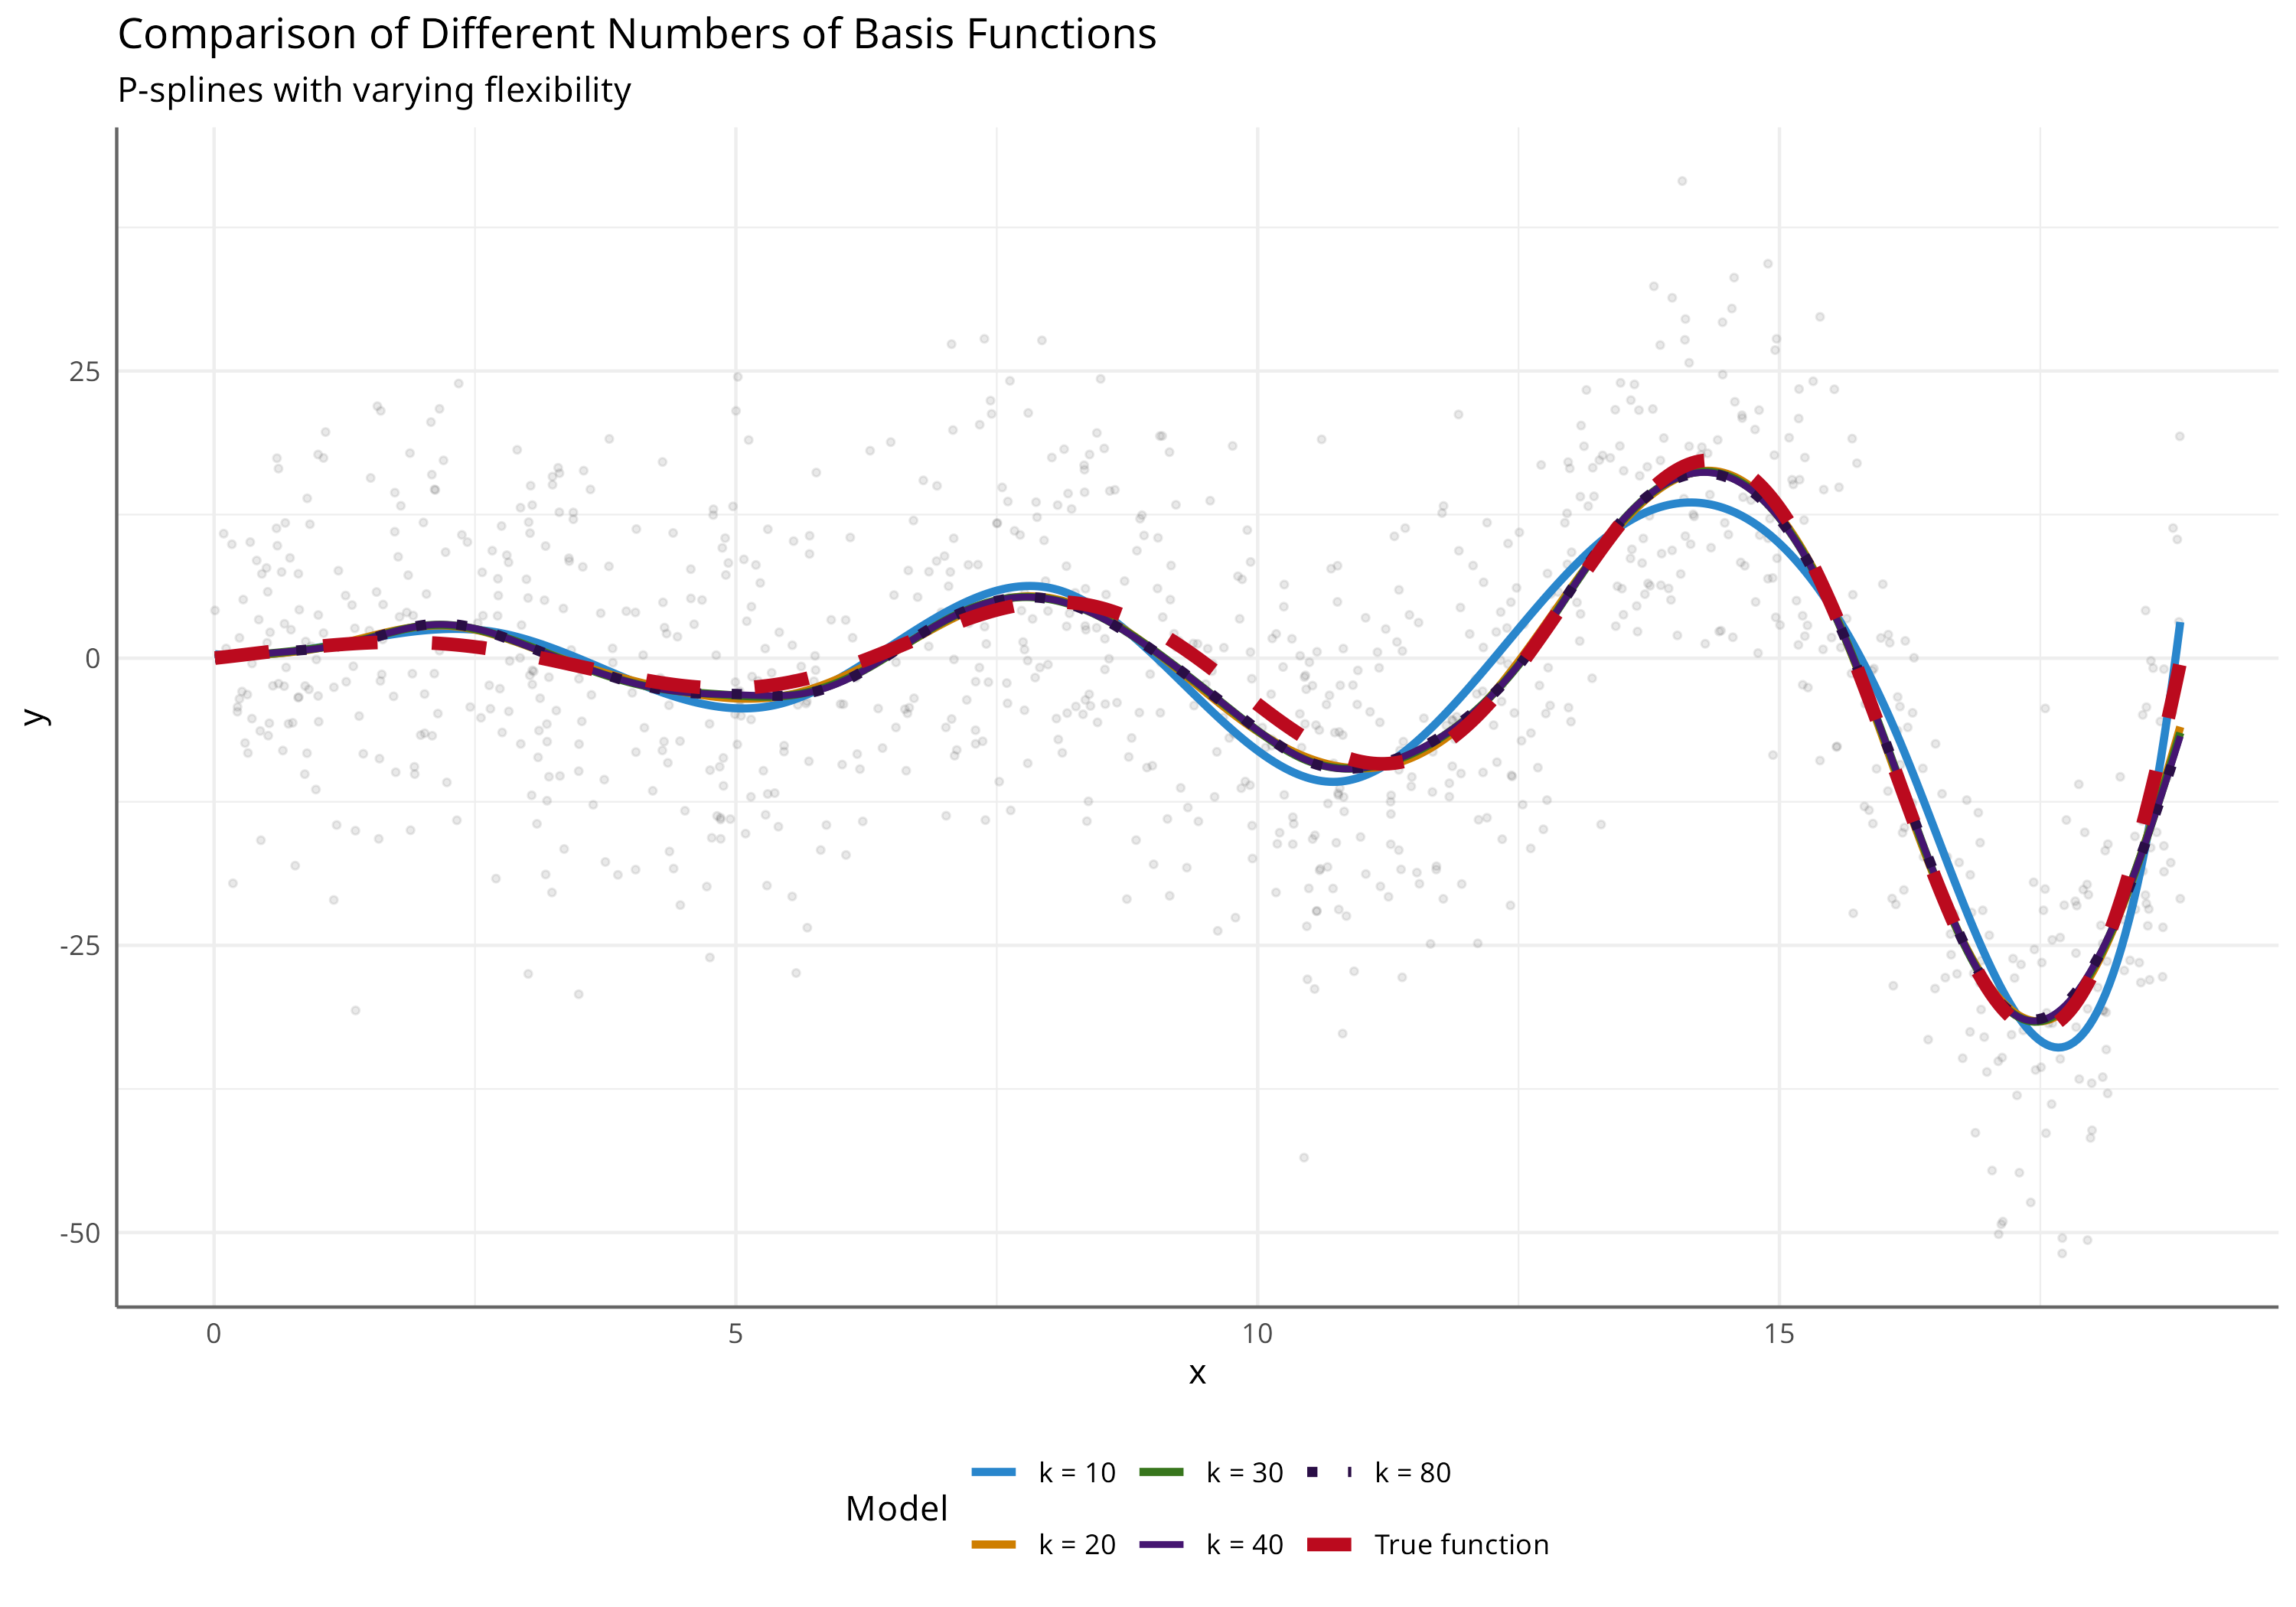
\includegraphics[width=0.8\columnwidth]{img1.png}
    \caption{Comparison of different numbers of basis functions}
    \label{fig:your_label}
    \vspace{-10pt}
\end{figure}

Finally, residual plot was analysed to determine as well as the residual distribution. From these plots it was determined that
residuals are univorm, homoscedastic with approximately normal distribution with Anderson-Darling Normality tests p-value being 0.114
which does not reject the normality hypothesis. The model explained 53.4\% of variance.

Overall, the model succesfully captured the non-linear relationwhip with the smoot term being highly significant (p-value <0.001; F = 60.11).

\begin{figure}[htbp]
    \centering
    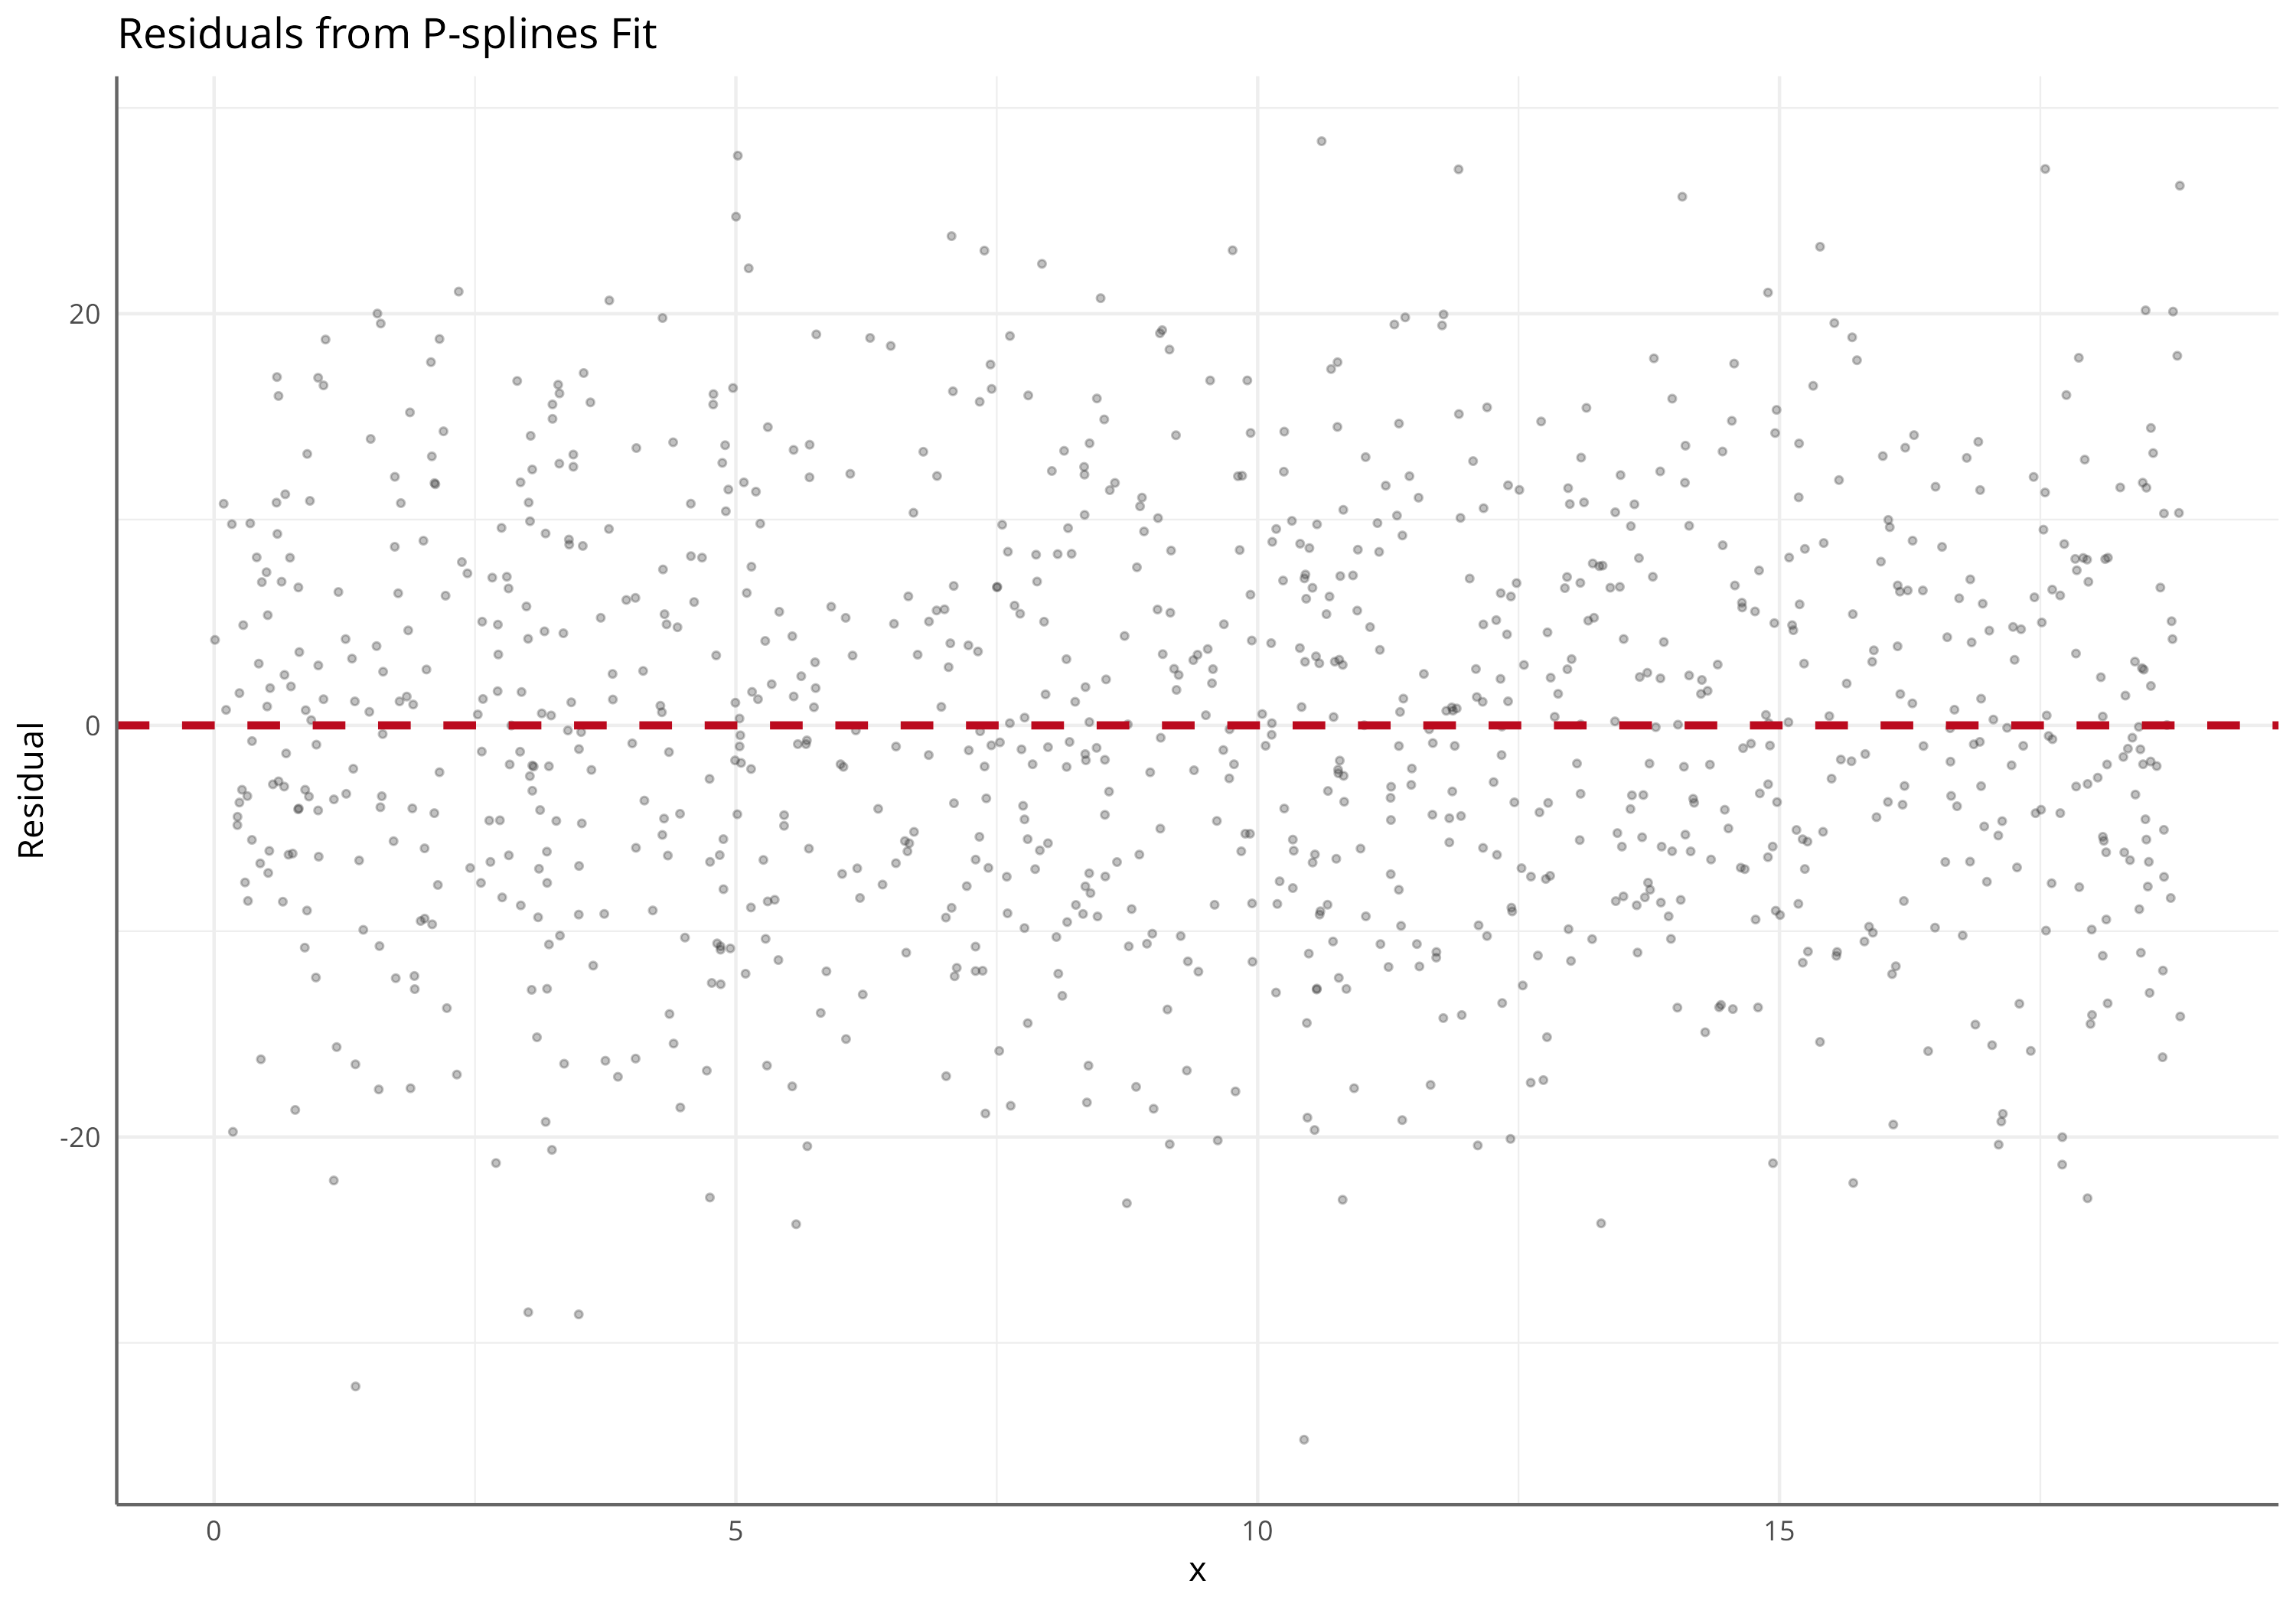
\includegraphics[width=0.40\columnwidth]{img2.png}
    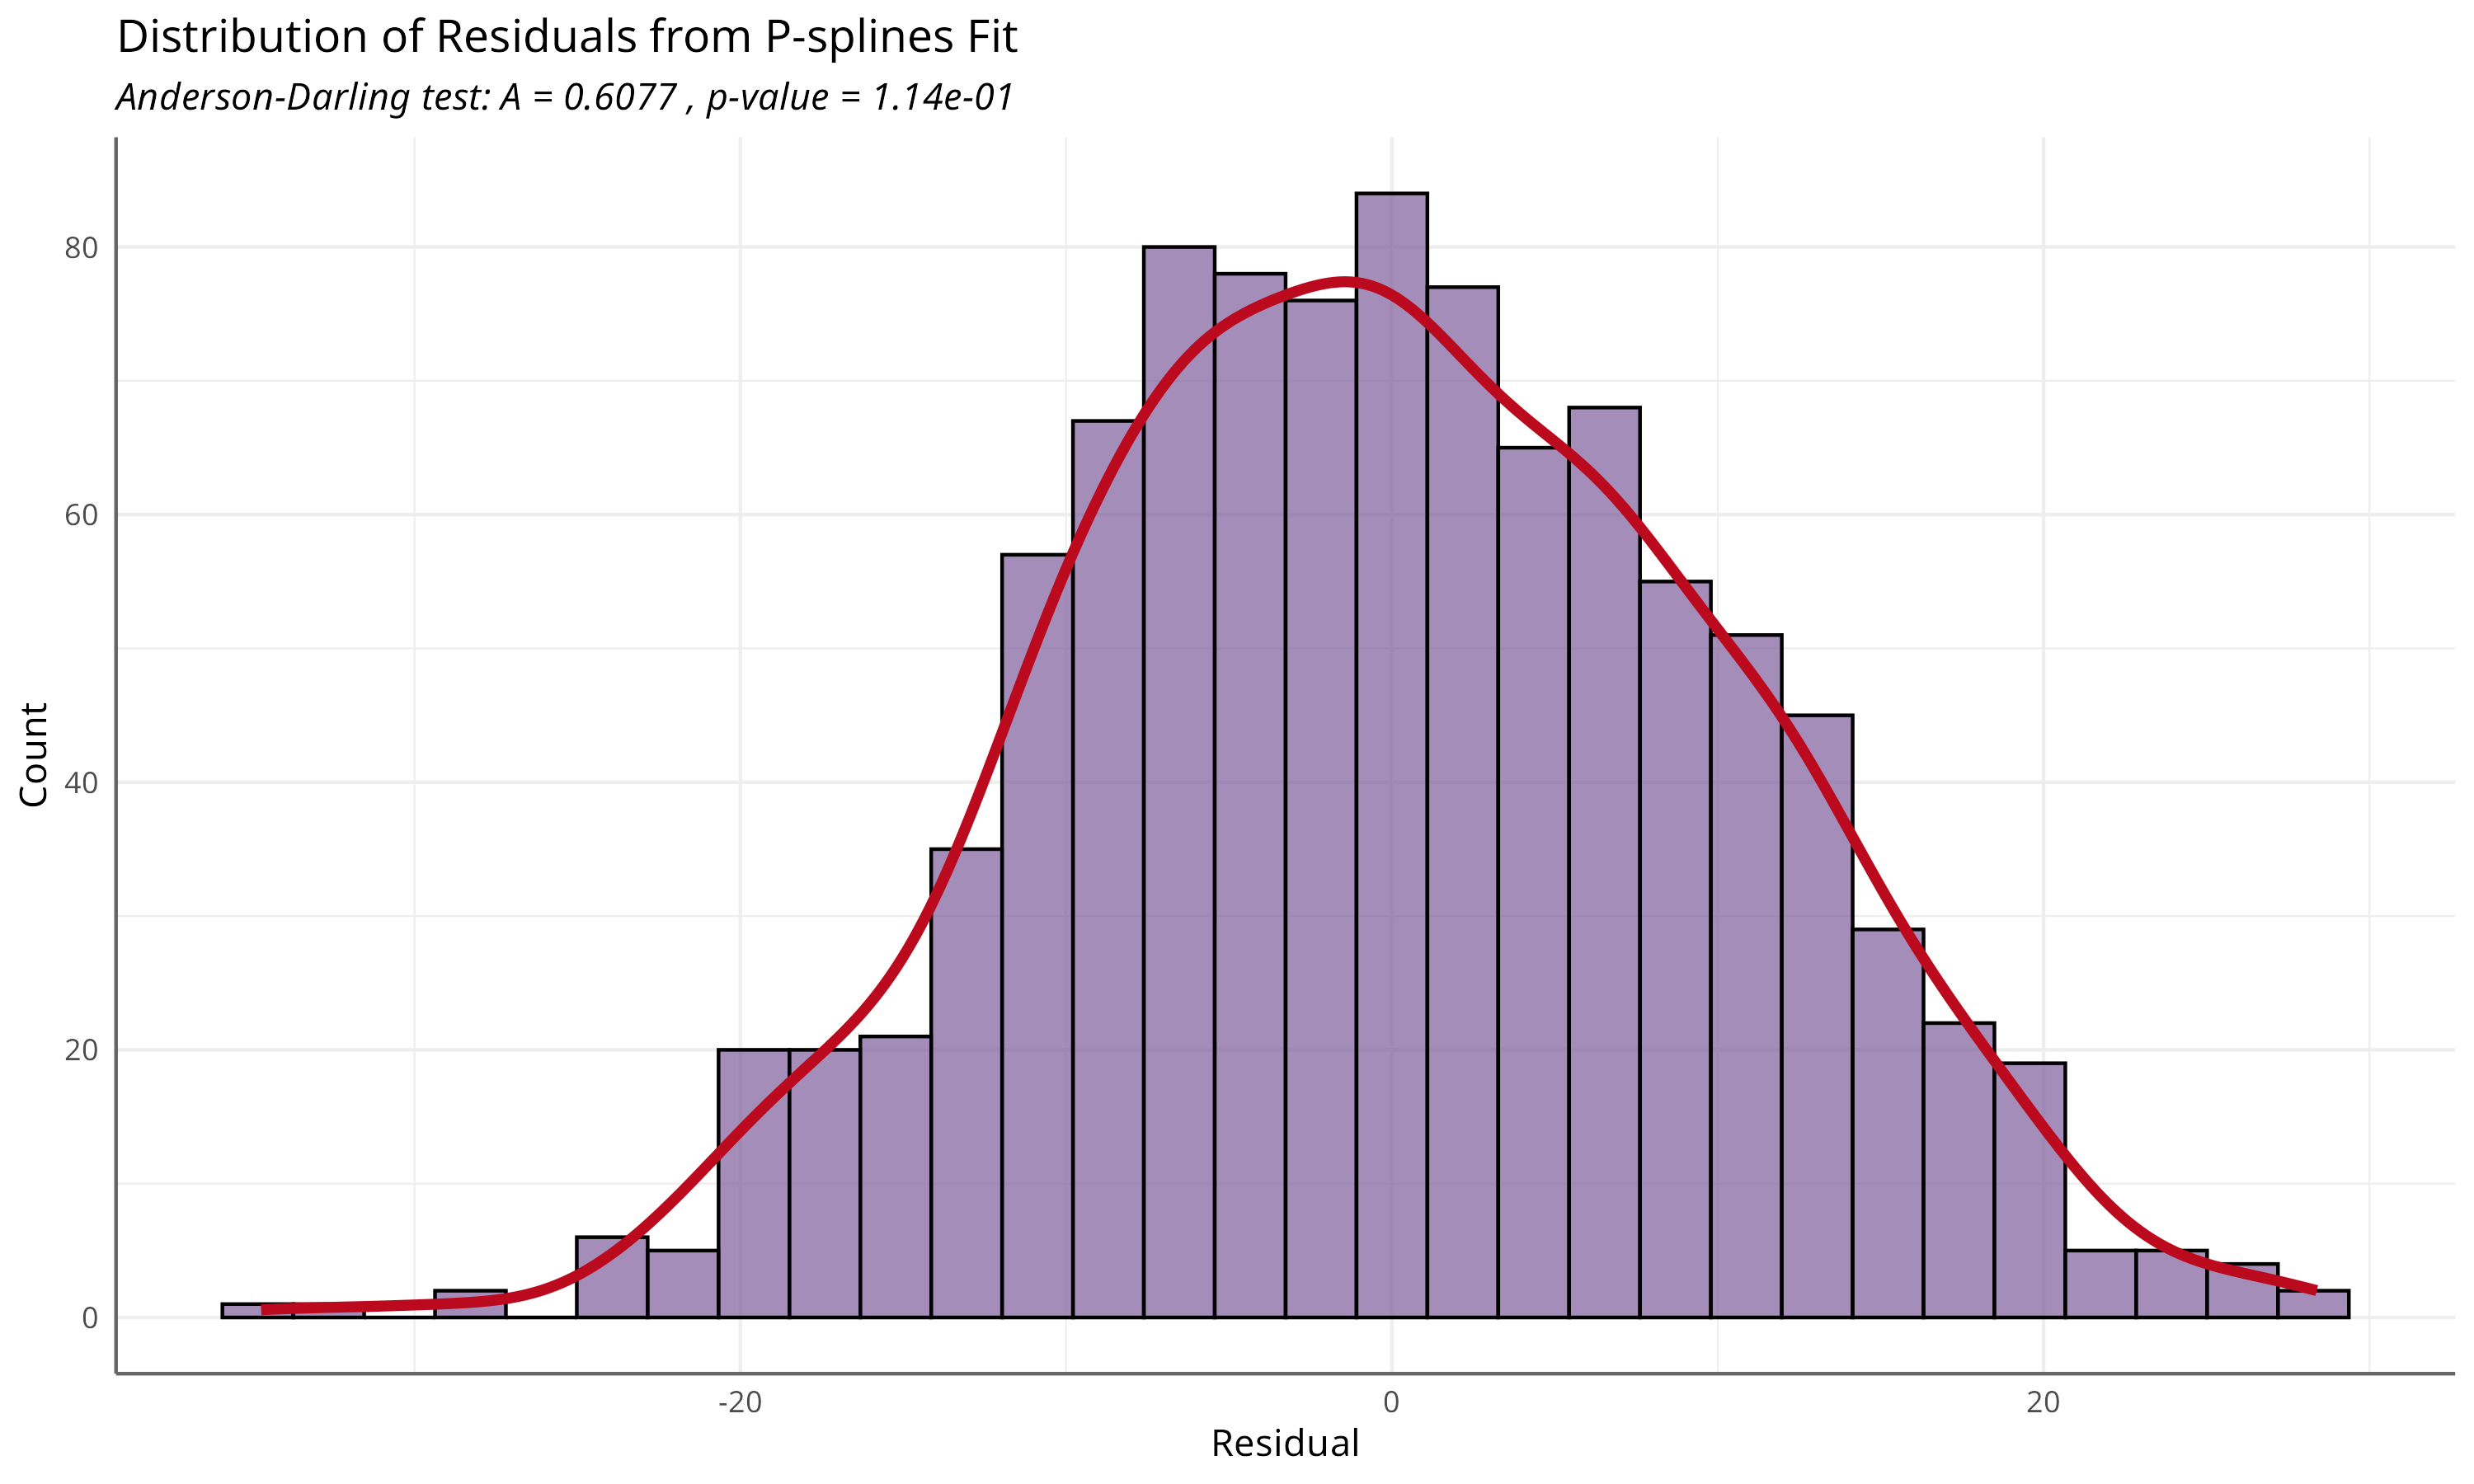
\includegraphics[width=0.40\columnwidth]{img3.png}
    \caption{Left image shows residual plot and right their distribution}
    \label{fig:both_images}
\end{figure}


\subsubsection{SVR Implementation}
Support Vector Regression was implemented using the \textbf{e1071} package, which interfaces with \textit{libsvm}. Two versions of the SVR model were explored: a base model using default parameters and a tuned model optimized using grid search.

This models were trained on scaled input data to avoid issues related to kernel sensitivity to variable magnitude.The base SVR model was trained using the radial basis function (RBF) kernel. A second, tuned SVR model was fitted by optimizing the $\epsilon$-insensitive margin and the regularization parameter $C$, with a search grid defined as $\epsilon \in [0, 1]$ and $C \in \{2^{-1}, 2^0, \dots, 2^7\}$. The best model was selected based on RMSE. 

Prediction accuracy was evaluated by comparing the fitted values to true values using a visual overlay (Figure 4) and RMSE scores across the linear model, base SVR, and tuned SVR (Table 1). The SVR tuned model clearly outperformed both the base SVR and linear regression models.

\begin{figure}[htbp]
    \centering
    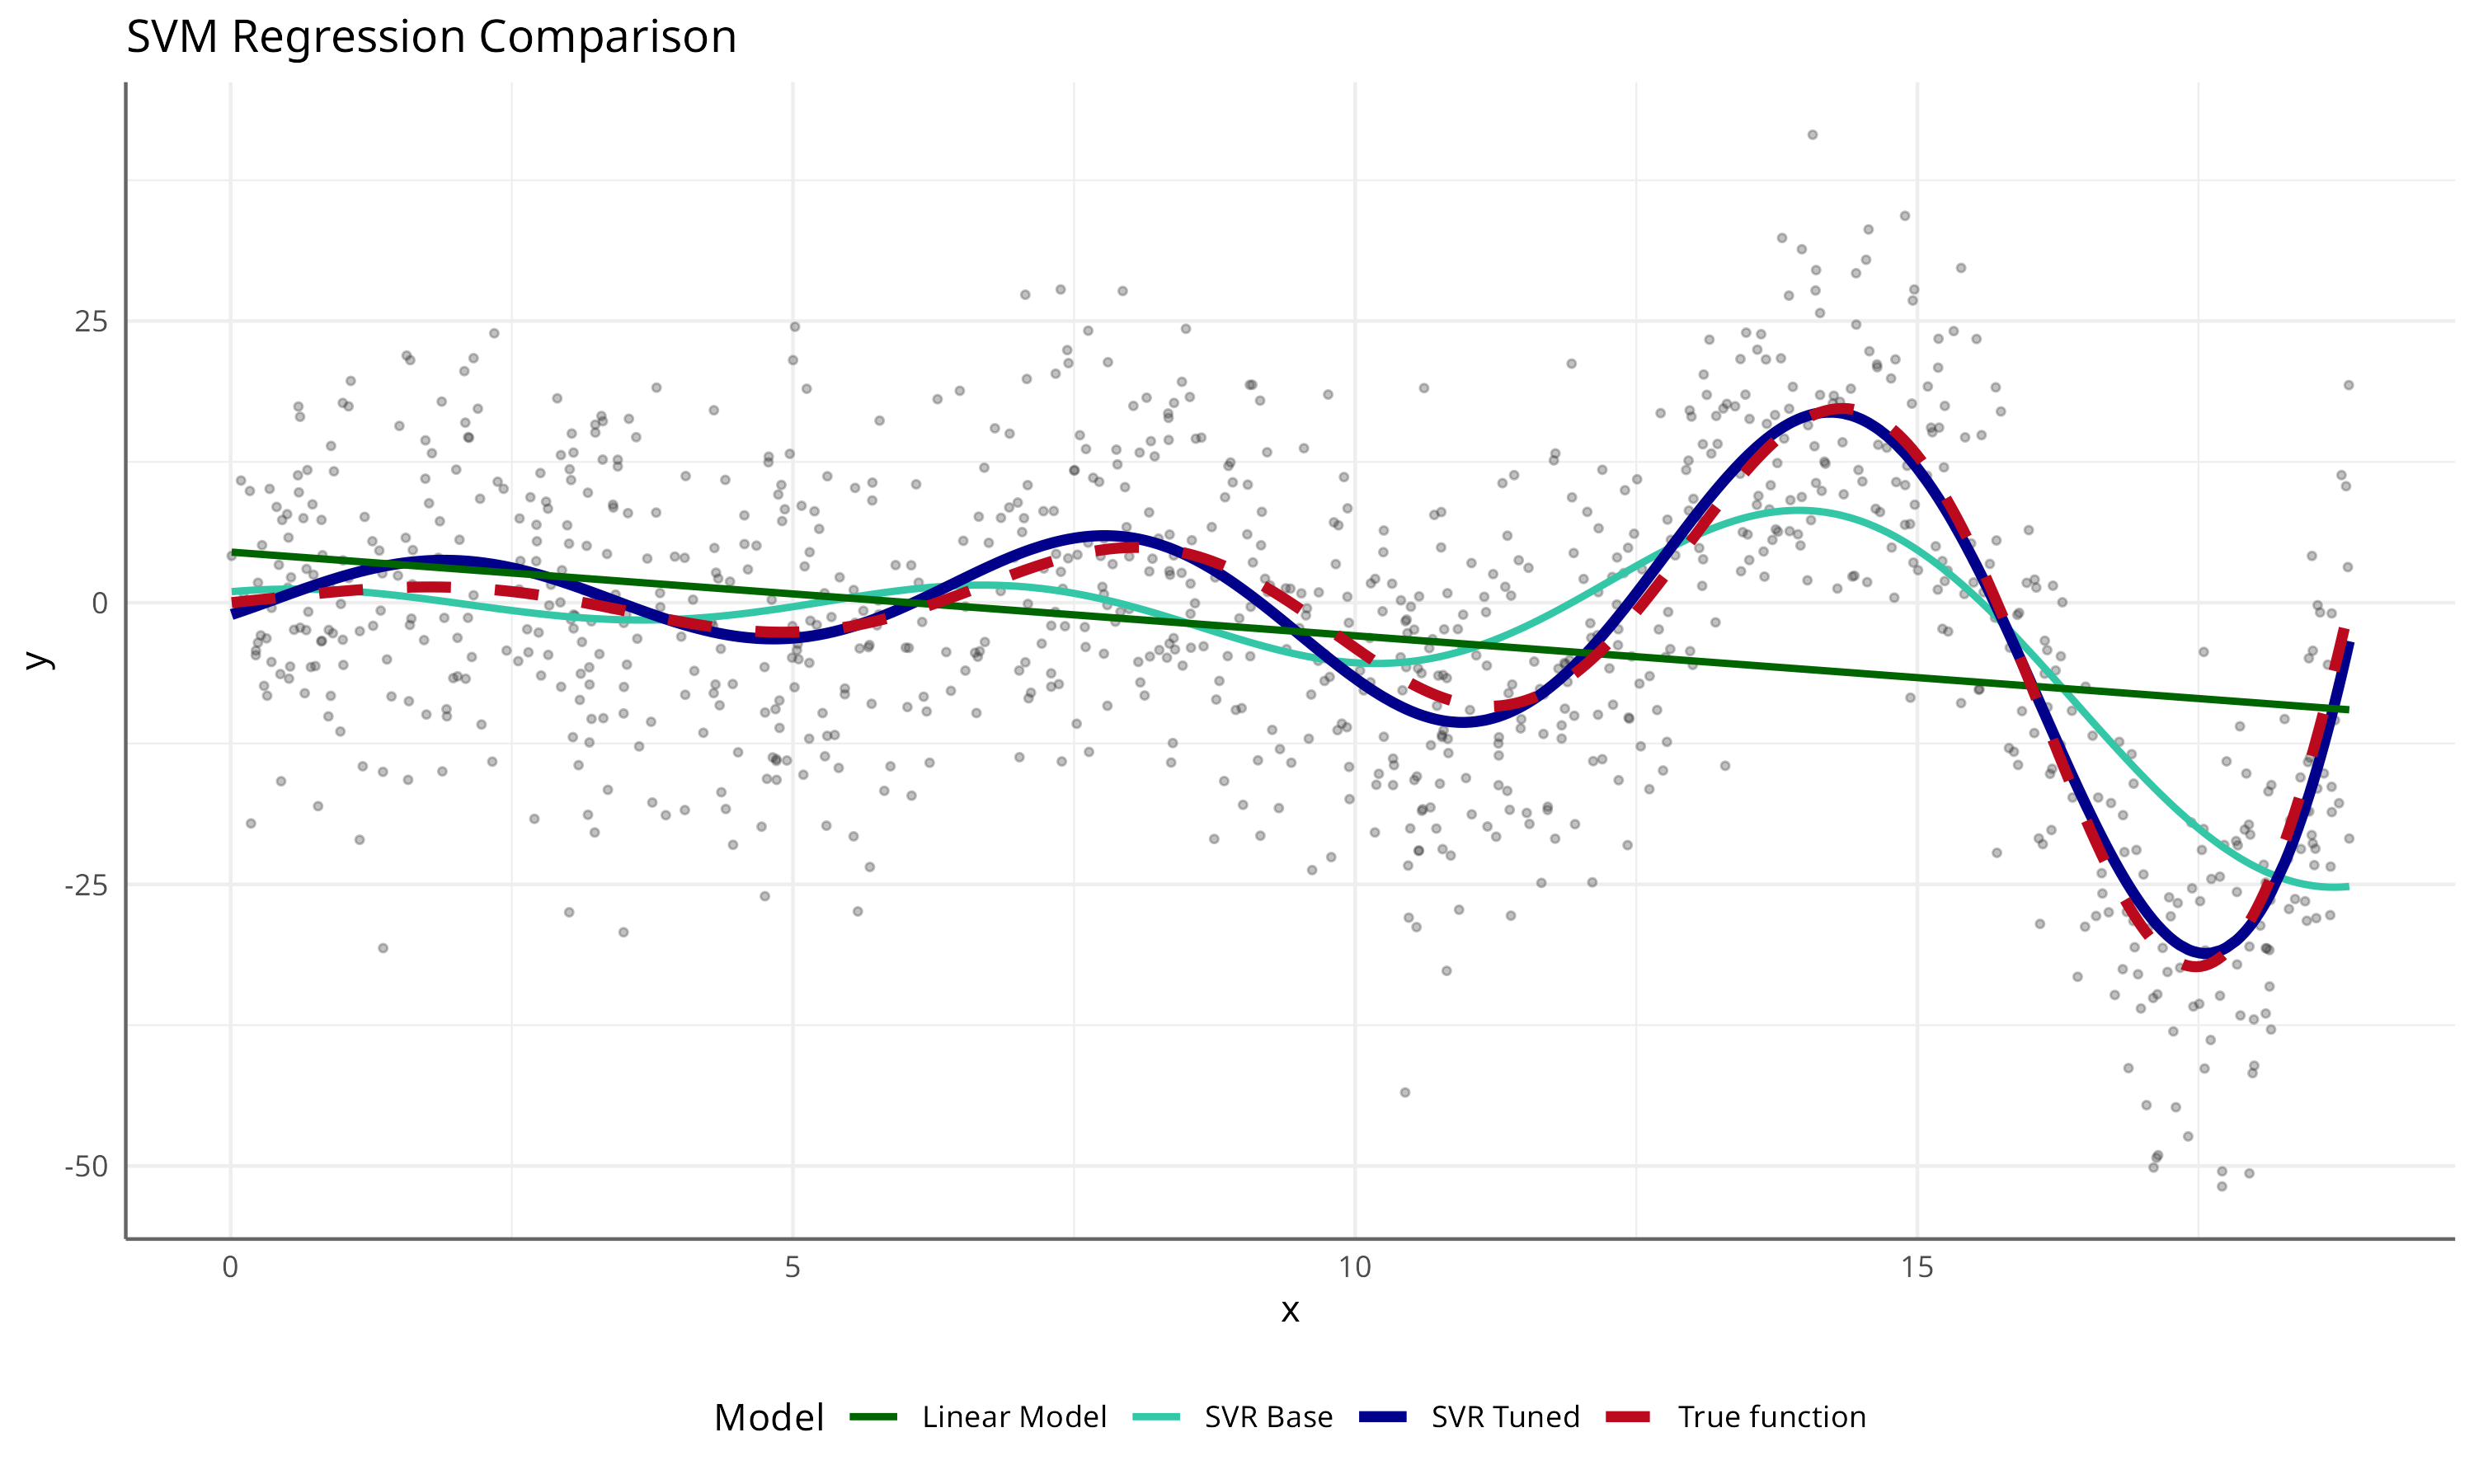
\includegraphics[width=0.8\columnwidth]{img4.png}
    \caption{Overlay of predicted vs actual values for Linear Regression, SVR Base, SVR Tuned models, and Actual Model}
    \label{fig:svr_overlay}
    \vspace{-10pt}
\end{figure}

\begin{table}[htbp]
    \centering
    \begin{tabular}{lcc}
    \hline
    \textbf{Model} & \textbf{RMSE} \\
    \hline
    Linear Regression & \texttt{14.350} \\
    SVR Base          & \texttt{11.720} \\
    SVR Tuned         & \texttt{10.220} \\
    \hline
    \end{tabular}
    \caption{Root Mean Squared Error (RMSE) comparison across models.}
    \label{tab:svr_rmse}
\end{table}

Residual analysis was performed to assess model performance beyond accuracy. The residuals from the tuned SVR model were plotted against fitted values and examined through histogram and density analysis (Figure~\ref{fig:svr_residuals}). The residuals appeared randomly scattered around zero and approximately normally distributed, supported by the Anderson-Darling test with a p-value of \texttt{0.076}, indicating no strong evidence against normality.

\begin{figure}[htbp]
    \centering
    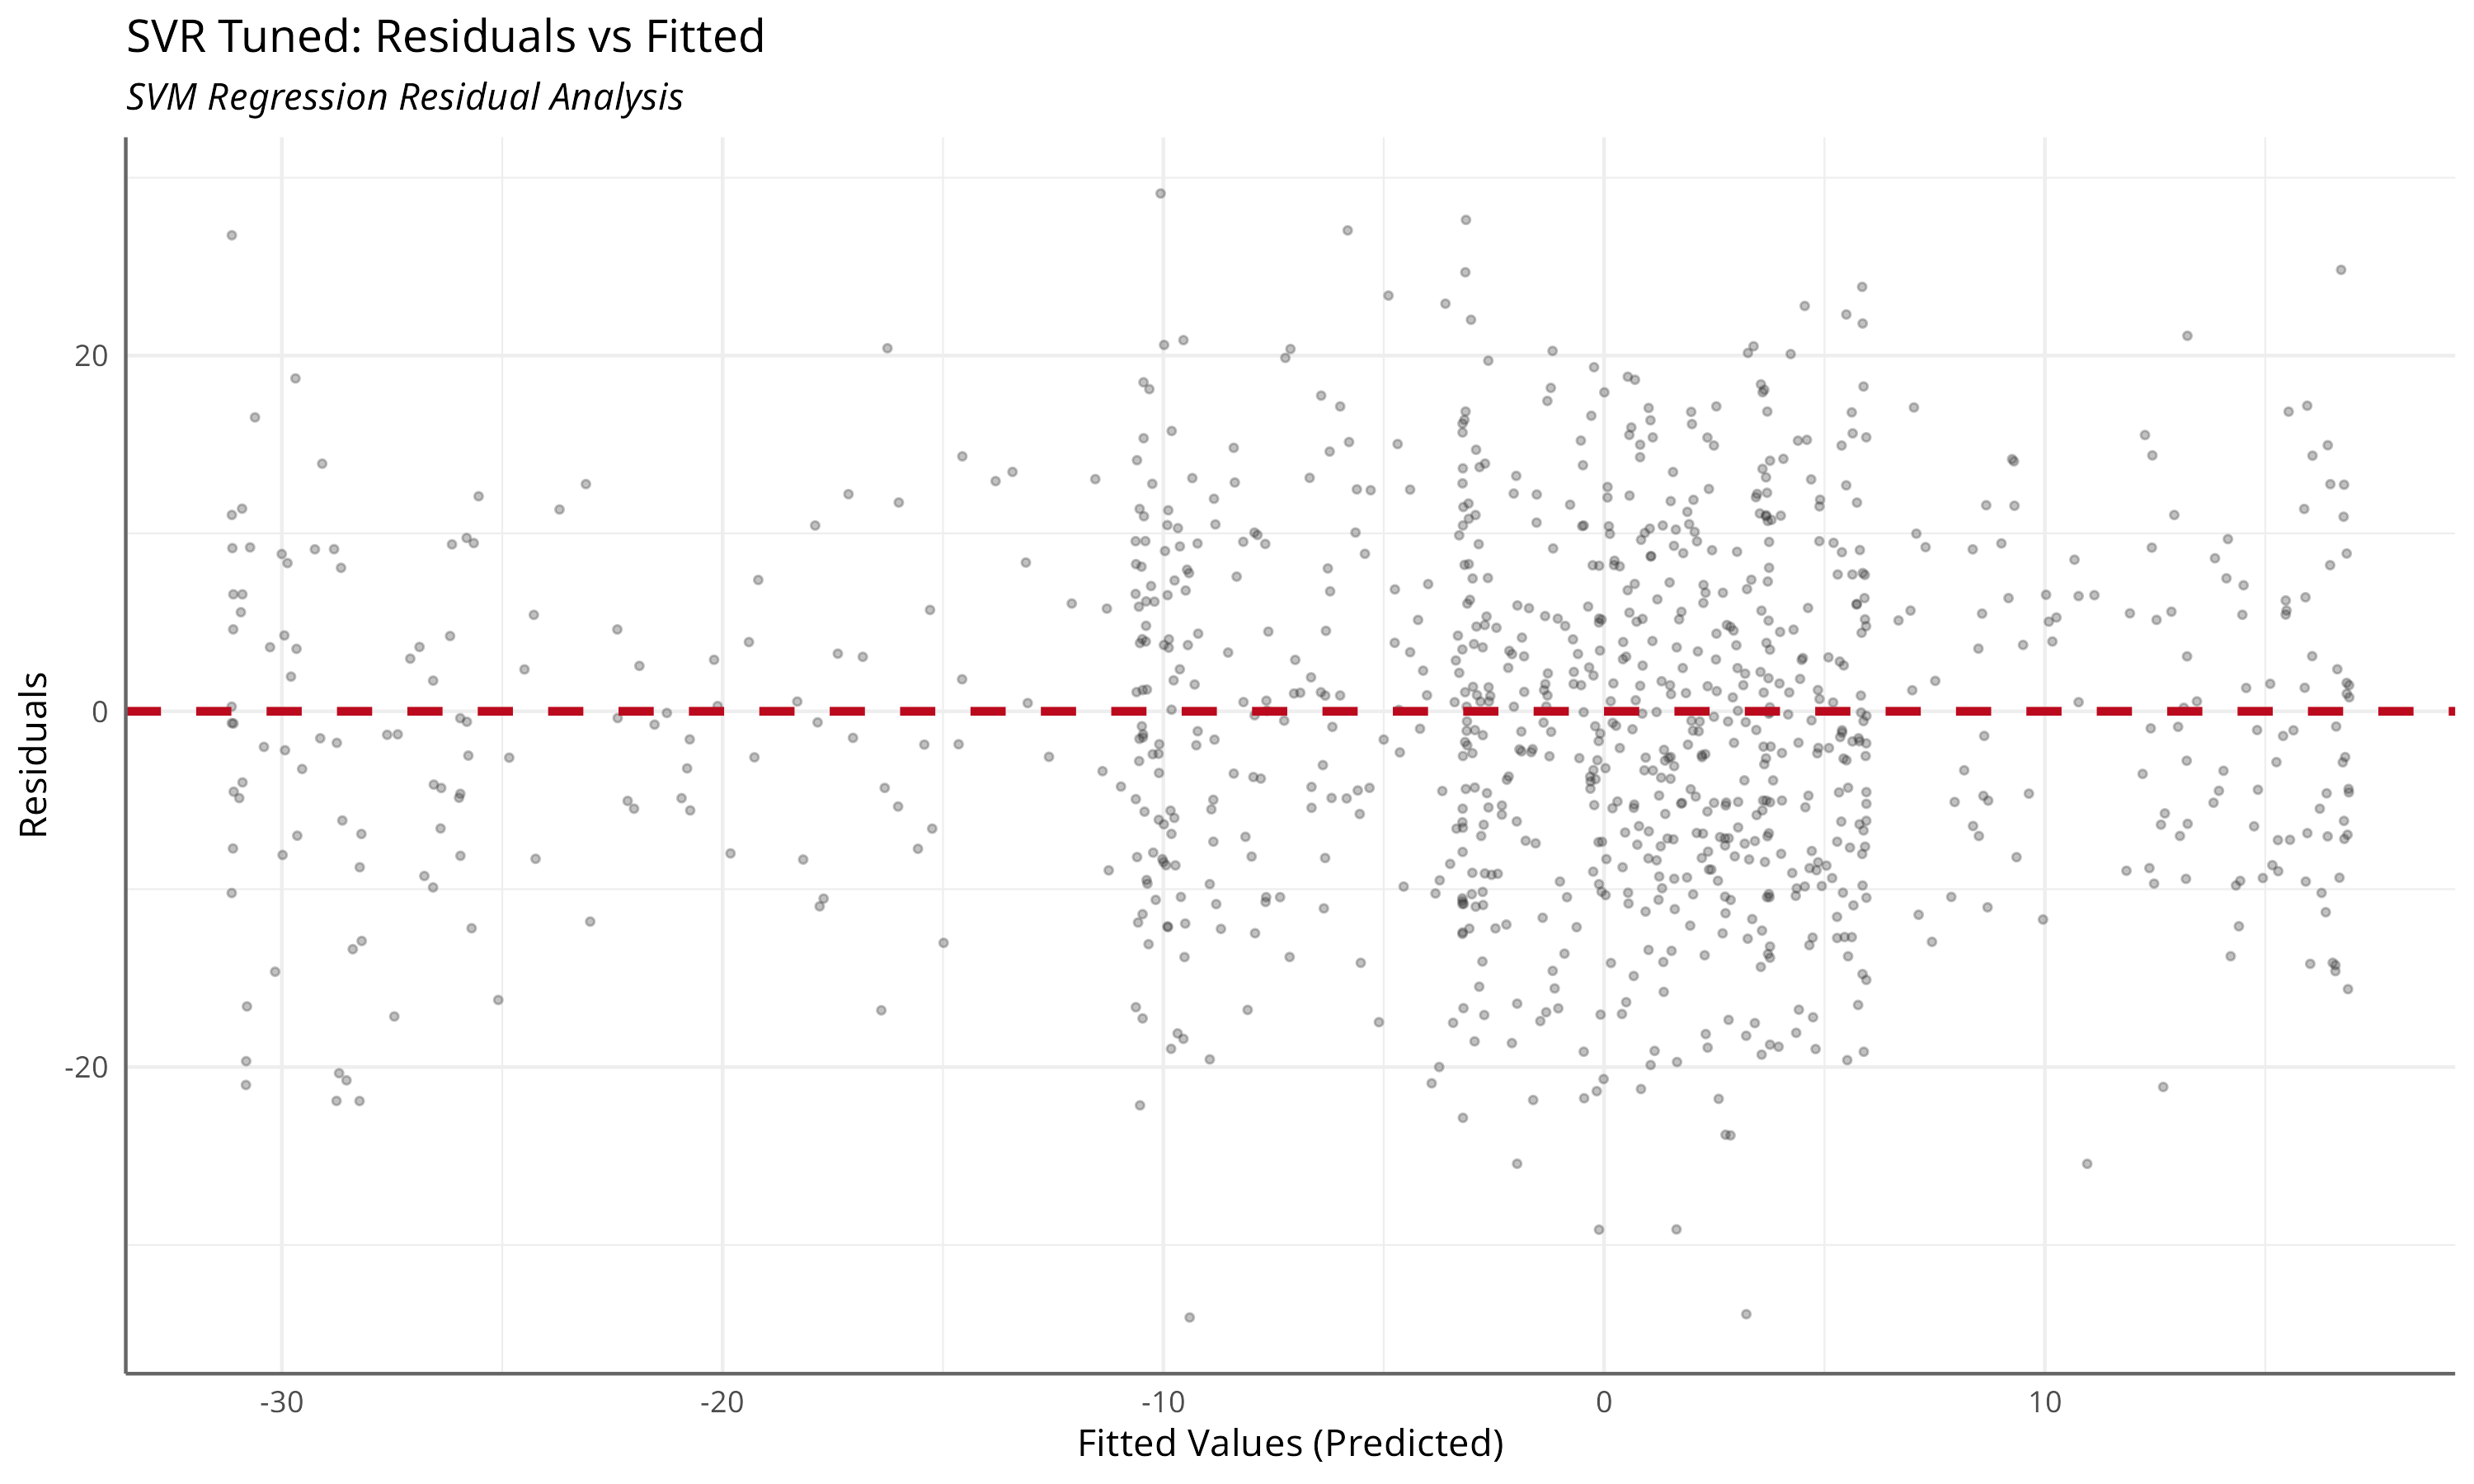
\includegraphics[width=0.40\columnwidth]{img5.png}
    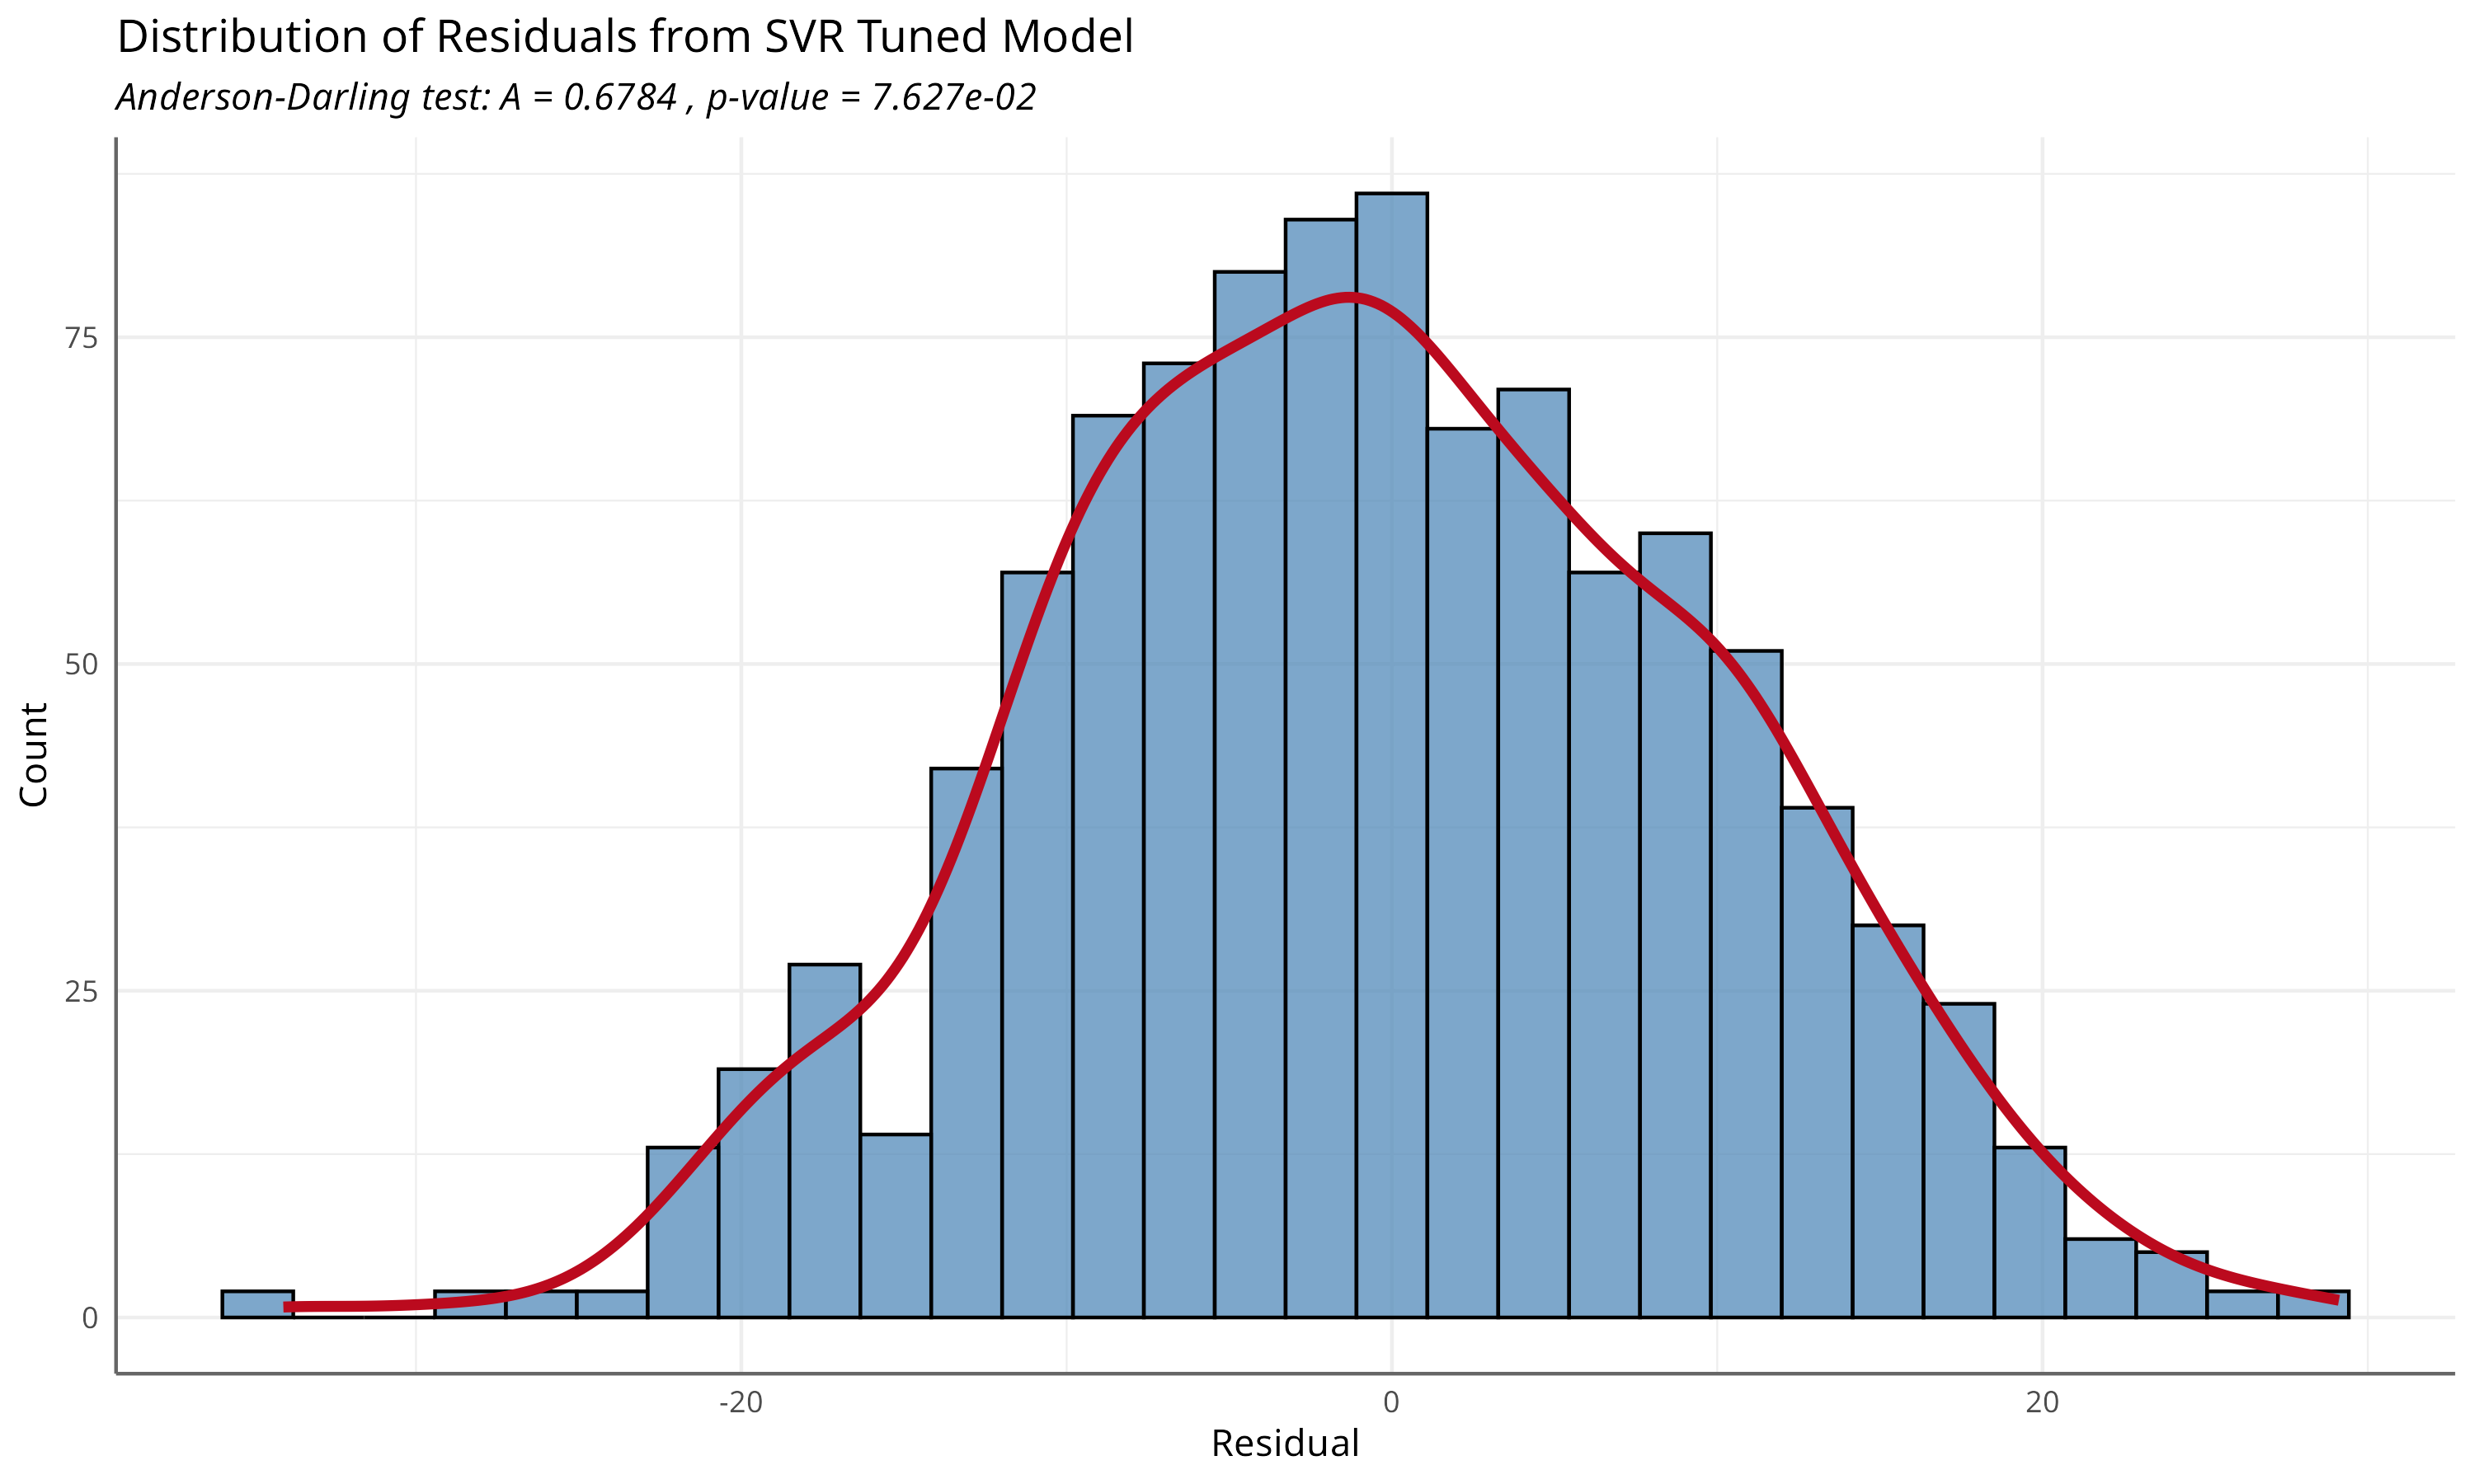
\includegraphics[width=0.40\columnwidth]{img6.png}
    \caption{Left: Residuals vs Fitted plot. Right: Residual distribution with Anderson-Darling test result.}
    \label{fig:svr_residuals}
\end{figure}

\subsubsection{Prediction Testing Method}

Firstly, a sample fo 200 new data was generated as a testing data set, meaning this data was not used for training of any models. We then made predictions using our models. Prediction interval(95\%) was calculated for both P-splines and SVMwhich was later used for calculating Prediction Interval Coverage Probability(PICP).

For P-splines, the Wood's package was used to calculate fit and standard error mmetrics. For SVM, a simulation method had to be used to achieve prediction interval. While using simulation on top of simulation reduces credibility of this aproach, this is the best solution given the lack of interval theory in SVM implementation. The number of bootstrap iteration was set to 1000 to calculate confidence intervals and later prediction intervals.

\subsection{Results}

The P-spline results suggest moderate prediction accuracy(RMSE = 10.178). The lower MAE(8.241) suggest there are not many extreme outliers with 54\% of explained variance.

\begin{table}[ht]
  \centering
  \caption{Goodness-of-fit and Prediction}
  \setlength{\tabcolsep}{4pt}
  \begin{tabular}{@{}lccc@{}}
    \toprule
      Model & RMSE & MAE & R-Sq  \\
    \midrule
      P-spline & 10.177 & 8.241 & 0.534 \\
      SVM Tuned & 10.220 & 8.277 & 0.530 \\ 
    \midrule
     Model & Pred-RMSE & PICP & Av. Interval Width \\
    \midrule
      P-spline & 10.024 & 0.97 & 40.553\\
      Svm Tuned & 10.034 & 0.97 & 40.267 \\
    \bottomrule
  \end{tabular}
\end{table}


\begin{figure}[htbp]
    \centering
    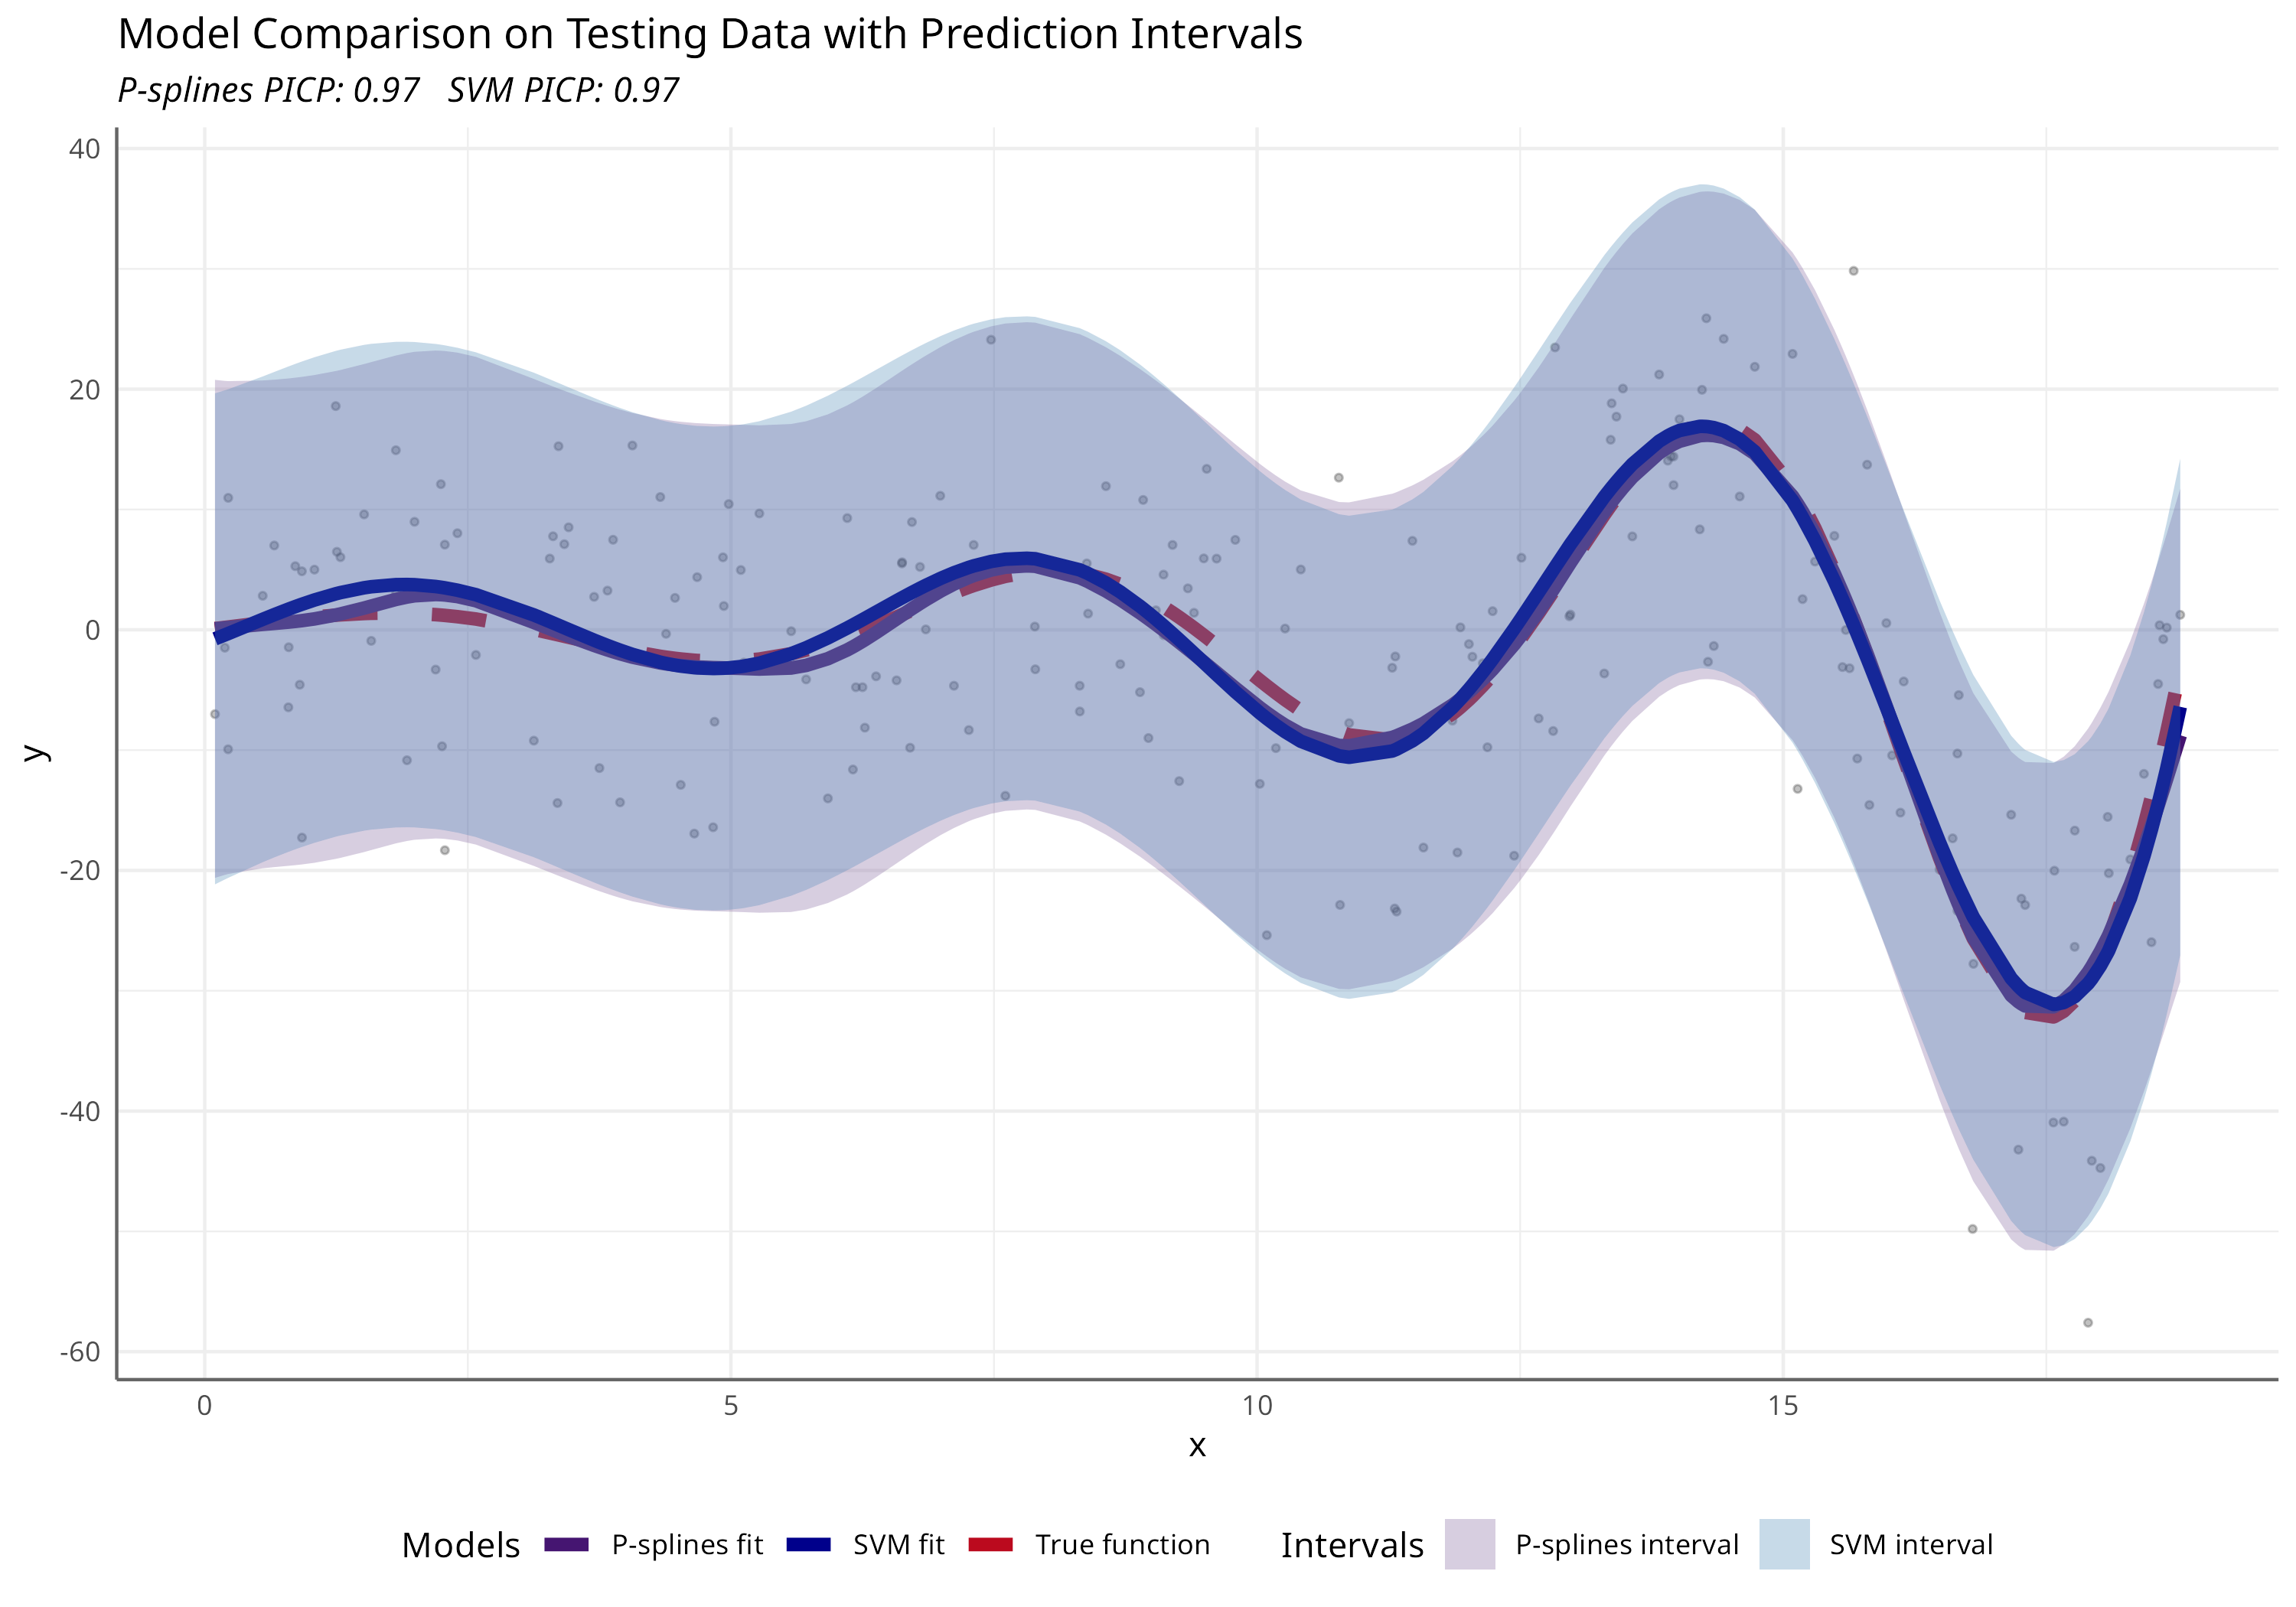
\includegraphics[width=0.8\columnwidth]{img7.png}
    \caption{Comparison predictive power between P-splines SVM Tuned models}
    \vspace{-10pt}
\end{figure}



% 4. CONCLUSION
\section{CONCLUSION}


\bibliography{citation}

\end{document}
